\documentclass[11pt]{article}
\usepackage[a4paper,margin=1in]{geometry}
\usepackage[T1]{fontenc}
\usepackage{amsmath,amssymb,booktabs,array,tabularx}
\usepackage{graphicx}
\usepackage[authoryear,round]{natbib}
\usepackage[hidelinks]{hyperref}
\title{Frequency and Coverage Damage under {LoRA} Adaptation:\\A Matched Four-Condition Decomposition on {BRACS} and {TCGA-UT}}
\author{Yannik Queisler}
\date{November 8, 2026}

\begin{document}
\raggedbottom
\widowpenalty=10000
\clubpenalty=10000
\setlength{\emergencystretch}{2em}
\maketitle
\begin{abstract}
\noindent Class imbalance changes two things at once: how strongly each class influences the training loss (frequency) and which patches of the rare classes are available at all (coverage). An earlier decomposition separated these two parts for a frozen encoder with a logistic-regression readout. The mitigation studies, however, adapted a Virchow2 encoder through low-rank adaptation (LoRA), so the frozen shares need not describe the learner whose recovery they are meant to explain. This experiment repeats the decomposition with the LoRA recipe of the mitigation studies on BRACS and TCGA-UT at an imbalance ratio of 100. Four matched conditions train fresh adapters and heads from the same initialization: a balanced reference, frequency only, coverage only, and both. Fixed loss weights change class influence without changing which patches are sampled. The contrasts give the total damage, its frequency and coverage parts, their interaction, and the recovery that restoring balanced class influence achieves under this recipe. The share of the total damage that this recovery represents serves as a conditional benchmark for rebalancing methods. On BRACS, training on the imbalanced patches with balanced class influence already costs 3.09 of the 5.07 lost points, and restoring balanced influence recovers 1.97 points, a share of 0.39 [0.24, 0.56]. On TCGA-UT, neither factor harms alone; their interaction carries 1.40 of the 1.58 lost points, and restoring balanced influence recovers all of it (share 1.01 [0.86, 1.22]). Logit adjustment in the mitigation studies recovered about the same amounts, so its incomplete BRACS recovery matches the coverage damage that remains when class influence is balanced.
\end{abstract}

\section{Motivation}
\label{sec:motivation}
On TCGA-UT and BRACS, an imbalance ratio of $\rho=100$ lowered the patient-macro balanced accuracy of a frozen Virchow2 encoder \citep{zimmermann2024virchow2} with a logistic-regression readout by 2.91 and 7.65 percentage points \citep{queisler2026causeTcga,queisler2026causeBracs}. Those studies split the damage into a part caused by the skewed class frequencies in the loss, a part caused by the thinner patch coverage of the rare classes, and their interaction. Frequency carried about two-fifths of the TCGA-UT damage and three-fifths of the BRACS damage.

The mitigation studies then trained a LoRA update \citep{hu2022lora} of the same encoder together with a linear head \citep{queisler2026mitigationMethods,queisler2026mitigationBracs,queisler2026mitigationTcga}. Several methods that act on class influence, such as logit adjustment, recovered between about two-fifths of the damage on BRACS and nearly all of it on TCGA-UT. Whether these recoveries are close to what removing the frequency part could achieve is not answered by the frozen shares: LoRA changes the encoder during training, so coverage and frequency may act differently. This experiment therefore asks: \emph{under the LoRA recipe of the mitigation studies, how much of the damage at $\rho=100$ comes from frequency, from coverage, and from their interaction, and how much does restoring balanced class influence recover?}

The question follows from mitigation results that were already observed. The answer is a descriptive benchmark for those results, not a prediction made before they were known.

\section{Design}
\label{sec:design}
The design fixes the data and training recipe of the mitigation studies and varies only two factors: the patch allocation the model trains on and the class shares that the loss gives each class.

\paragraph{Data.} Both datasets use the three patient-disjoint splits and the ten allocation draws per split of the mitigation studies, giving 30 blocks per dataset. BRACS \citep{brancati2022bracs} has seven classes; each block trains on 10 patients per class and 2,240 patches. TCGA-UT \citep{komura2022universalEncoding} has 30 classes; each block trains on 20 patients per class and 19,200 patches. Within a block, the balanced allocation $r1$ gives every class the same number of patches, and the imbalanced allocation $r100$ gives the classes exponentially decreasing patch counts with a ratio of 100 between the largest and smallest class. Both allocations reuse the patients, patch order, and class-to-rank assignment of the mitigation studies. Validation and test patients, class order, preprocessing, and the evaluation metric are unchanged.

\paragraph{Conditions.} Table~\ref{tab:arms} defines the four conditions. The frequency-only condition F trains on the balanced patches but weights the loss so that each class has the influence it would have under $r100$. The coverage-only condition C trains on the imbalanced patches but weights the loss so that every class has the same influence. The balanced reference B and the both condition R need no reweighting.

\begin{table}[htbp]
\centering
\small
\renewcommand{\arraystretch}{1.15}
\begin{tabular}{@{}llll@{}}
\toprule
Condition & Patch allocation & Class shares in the loss & Varies \\
\midrule
B: balanced reference & $r1$ & uniform & neither \\
F: frequency only & $r1$ & realized $r100$ shares & frequency \\
C: coverage only & $r100$ & uniform & coverage \\
R: both & $r100$ & realized $r100$ shares & both \\
\bottomrule
\end{tabular}
\caption{The four matched conditions. Each condition trains its own LoRA adapters and linear head from the pretrained encoder. The target $r100$ shares are the class shares realized by the block's own imbalanced allocation, not an idealized profile.}
\label{tab:arms}
\end{table}

\paragraph{Loss weights.} Let class $c$ have $n_c$ of the $N$ training patches, and let $q_c$ be the share the loss should give it. Every patch of class $c$ receives the fixed weight
\begin{equation}
w_c = \frac{q_c}{n_c / N},
\label{eq:weights}
\end{equation}
and the loss of a batch of size $b$ is $\frac{1}{b}\sum_{i} w_{y_i}\,\ell_i$, where $\ell_i$ is the cross-entropy of patch $i$. The weights average to one over the training patches, so B and R reduce to ordinary cross-entropy. The batch loss divides by the batch size rather than by the sum of the weights in the batch; a batch that happens to contain no rare-class patch therefore keeps the same scale as any other batch.

\paragraph{Pairing.} Every condition samples patches uniformly with replacement from its own allocation. B and F draw the same sequence of patch positions, and so do C and R. Changing the class shares in the loss therefore does not change which patches are seen. Within a block, all four conditions also start from the same adapter and head weights: a random seed derived from the split and draw resets every random number generator before each fit. Different blocks use different seeds. Each fit records digests of its initial weights and of the sampled positions, and a technical check confirms that they agree within each block before any results are pooled.

\paragraph{Training.} The recipe is that of the mitigation studies: LoRA rank 8, scaling 16, and no dropout on every attention projection; a linear head; batch size 256; AdamW with learning rate $10^{-4}$ and weight decay $10^{-4}$; a cosine schedule; and 600 (BRACS) or 2,400 (TCGA-UT) updates. Images are decoded deterministically without augmentation. The recipe is held fixed for all four conditions; it is not tuned for any of them. One block per split is trained first to check the implementation and the training behaviour; this check concerns numerical and technical soundness only and never the size or direction of an effect.

\section{Estimands}
\label{sec:estimands}
Let B, F, C, and R denote the patient-macro balanced accuracies of the four conditions, pooled over the 30 blocks of a dataset, in percentage points. Damage is reported as a positive number when imbalance lowers accuracy:
\begin{align}
D &= B - R && \text{total damage,} \\
D_F &= B - F && \text{frequency-only damage,} \\
D_C &= B - C && \text{coverage-only damage,} \\
I &= D - D_F - D_C && \text{interaction.}
\end{align}
A positive interaction means that the two parts together cause more damage than their sum. Restoring balanced class influence on the imbalanced patches moves the model from R to C. Its recovery and the corresponding share of the total damage are
\begin{equation}
G = C - R = D_F + I, \qquad h = \frac{G}{D} = 1 - \frac{D_C}{D}.
\label{eq:share}
\end{equation}
The absolute contrasts are the primary results; $h$ is secondary. $h$ is reported with its paired interval and is not truncated to $[0,1]$. A numerical share is interpreted only if the point estimate of $D$ is at least one percentage point and its 95\% interval lies strictly above zero; otherwise only the absolute contrasts are interpreted. Replicates with a non-positive denominator are counted and reported, never discarded, and the random denominator is never replaced by its observed value.

\section{Inference}
\label{sec:inference}
Uncertainty follows the mitigation studies. Bayesian bootstrap weights on test patients \citep{rubin1981bayesian} are combined with resampling of the ten draws within each split, and each split receives equal weight. The patient weights are shared across the three splits, so a patient who appears in more than one test split carries one weight in every replicate. All four conditions share the patient weights and the resampled draws, so every contrast is a difference of paired distributions. Intervals are 95\% percentile intervals from 10,000 replicates; the observed estimate never enters an interval. They are marginal estimation intervals for each quantity, not a simultaneous test of all components.

Two diagnostics show where the uncertainty comes from. The patient-only interval keeps every draw at equal weight and resamples only patients; the draw-only interval keeps the observed patients and resamples only draws. Neither replaces the full interval, and their widths do not add. Because each draw has one random seed, the draw-only spread includes initialization variation as well as allocation variation. Per-split estimates show whether a finding depends on one patient split.

\section{Interpretation}
\label{sec:interpretation}
The experiment yields a matched decomposition for one learner and one training recipe. $G$ is the recovery that restoring balanced class influence achieves when nothing else changes; it is not an upper bound for augmentation, other losses, or better optimization, and $D_C$ is not an irreducible information limit. The decomposition supports a conditional statement: a method that removes the frequency-related damage and leaves the coverage residual unchanged should recover close to $G$, that is, a share close to $h$. Comparisons with the mitigation results are descriptive, and they distinguish a method's plain recovery from its recovery after subtracting its gain on balanced data.

\IfFileExists{results.tex}{\section{Results}
\label{sec:results}
All 240 fits completed and passed the technical checks. Within every block, the four conditions started from identical weights, B/F and C/R pairs drew identical patch sequences, and the loss targets matched the paired imbalanced allocation. The balanced reference B and condition R reproduce the cross-entropy runs of the mitigation studies: B is 36.49 on BRACS and 71.45 on TCGA-UT (earlier 36.53 and 71.51), and total damage is 5.07 and 1.58 percentage points (earlier 4.95 and 1.56). Table~\ref{tab:results} lists all accuracies and contrasts; Figure~\ref{fig:components} shows the contrasts with their intervals.

\begin{table}[htbp]
\centering
\small
\renewcommand{\arraystretch}{1.15}
\begin{tabular}{@{}lll@{}}
\csname @@input\endcsname arm_table.tex
\end{tabular}
\caption{Coverage-only damage accounts for most estimated BRACS damage; the interaction accounts for most on TCGA-UT, where both single-factor intervals span zero. Rows one to four are patient-macro balanced accuracies (\%); the remaining rows are contrasts in percentage points, with positive damage meaning lower accuracy under imbalance. Brackets give 95\% paired bootstrap intervals.}
\label{tab:results}
\end{table}

\begin{figure}[htbp]
\centering
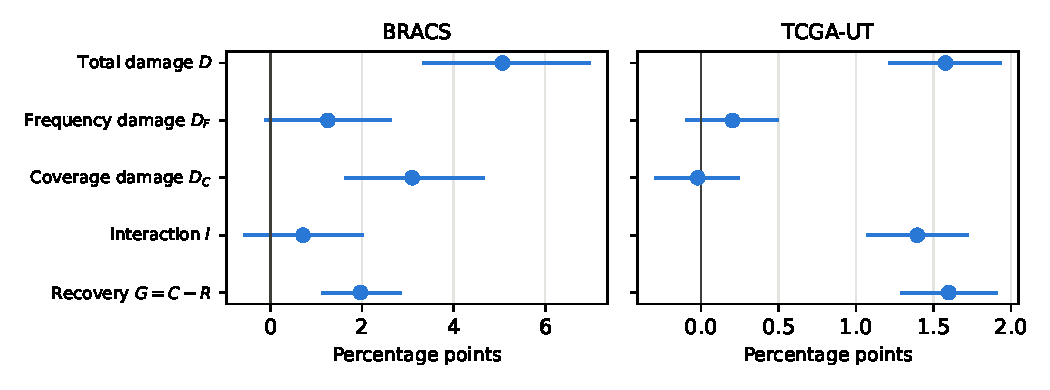
\includegraphics[width=\textwidth]{component_figure.pdf}
\caption{Damage components at $\rho=100$ under low-rank adaptation (LoRA), with 95\% paired intervals. On BRACS, coverage-only damage is the only resolved component besides the total; on TCGA-UT, the interaction is resolved and both single-factor damages are close to zero. The horizontal scales differ between panels.}
\label{fig:components}
\end{figure}

\paragraph{BRACS.} Training on the imbalanced patches with balanced class influence costs 3.09 [1.62, 4.67] points, about three-fifths of the total damage of 5.07 [3.32, 6.98]. Skewing class influence on the balanced patches costs 1.26 [$-0.13$, 2.64] points, and the interaction is 0.72 [$-0.58$, 2.03]; neither interval excludes zero. Restoring balanced class influence on the imbalanced patches recovers $G = 1.97$ [1.12, 2.87] points, a share $h = 0.39$ [0.24, 0.56] of total damage. The share meets the interpretation criteria: total damage exceeds one point and its interval lies above zero. No bootstrap replicate has a non-positive denominator. Across the three splits, coverage-only damage ranges from 2.69 to 3.77 points and the share from 0.36 to 0.42.

\paragraph{TCGA-UT.} Both single-factor damage estimates are close to zero and their intervals span zero: frequency-only damage is 0.20 [$-0.10$, 0.50] and coverage-only damage is $-0.02$ [$-0.30$, 0.25] points. Together they cost 1.58 [1.21, 1.94] points, with the interaction of 1.40 [1.07, 1.73] accounting for most of the estimated damage. Restoring balanced class influence recovers $G = 1.60$ [1.29, 1.91] points, a share $h = 1.01$ [0.86, 1.22] of the damage. The share interval includes full recovery but also allows incomplete recovery or recovery beyond the balanced reference. The coverage-only interval spans small gains and losses rather than establishing exact equality. Across the three splits, the interaction ranges from 1.30 to 1.55 points and the share from 0.95 to 1.08.

\paragraph{Sources of uncertainty.} Resampling only patients or only draws gives intervals of similar width, both narrower than the full intervals. On BRACS, for example, frequency-only damage has a patient-only interval of [0.62, 1.94] and a draw-only interval of [0.15, 2.34]; on TCGA-UT, the interaction has corresponding intervals of [1.23, 1.56] and [1.15, 1.63]. Uncertainty therefore comes from both the finite test cohort and variation between allocation draws, which here also includes random initialization.

\paragraph{Comparison with the frozen readout.} The decomposition differs from that of the frozen-encoder logistic-regression readout on the same patients \citep{queisler2026causeBracs,queisler2026causeTcga}, mainly in frequency-only damage. On BRACS, the frozen readout lost 4.47 points to frequency and 3.29 to coverage; under LoRA, frequency-only damage falls to 1.26, while coverage-only damage remains similar at 3.09. On TCGA-UT, the frozen readout lost 1.20 points to frequency, 0.53 to coverage, and 1.18 to the interaction; under LoRA, both single-factor damage estimates are close to zero, while an interaction of similar size, 1.40, remains. The two learners also differ in loss, optimizer, and training length, so this comparison does not isolate an effect of LoRA.

\paragraph{Comparison with the mitigation methods.} Figure~\ref{fig:recovery} compares recoveries from the mitigation studies with the benchmark $G$. These recoveries use the earlier runs and their own estimate of total damage, so the comparison is descriptive. On BRACS, training-time and post-hoc logit adjustment recover 1.96 and 1.94 points, close to $G = 1.97$. Curriculum of data augmentation (CUDA) recovers more, 2.59 points, but subtracting its gain on balanced data leaves only 1.20 points, below the benchmark in point estimate. On TCGA-UT, training-time and post-hoc logit adjustment recover 1.54 and 1.41 points, within the interval for $G = 1.60$. The estimates are descriptively similar to the benchmark; this comparison does not establish equal recovery.

\begin{figure}[htbp]
\centering
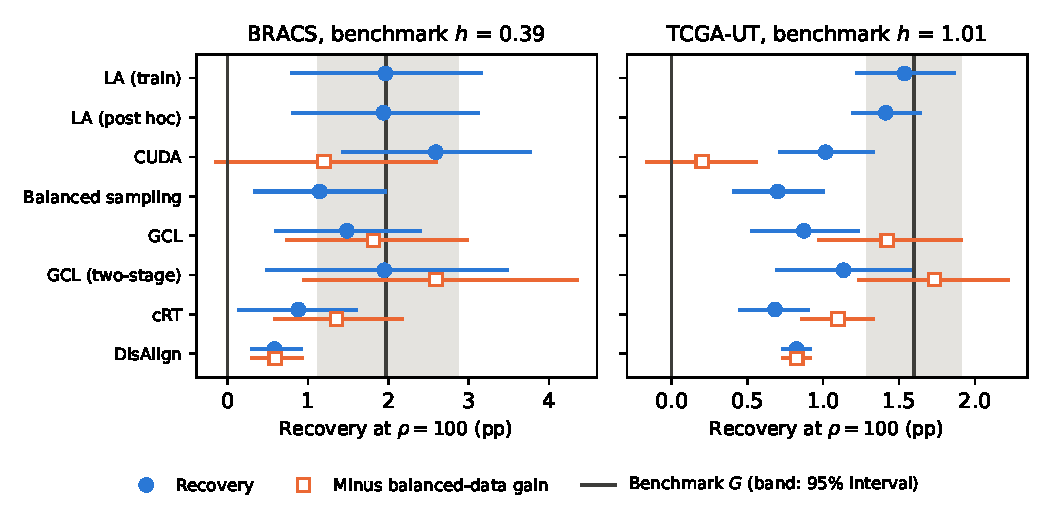
\includegraphics[width=\textwidth]{recovery_figure.pdf}
\caption{Logit adjustment gives descriptively similar recovery to restoring balanced class influence on both datasets. Points show each mitigation method's recovery at $\rho=100$ from the mitigation studies (filled) and, where defined, the recovery after subtracting its gain on balanced data (open). The vertical line and band show this experiment's benchmark $G$ and its 95\% interval; the panel titles give the share $h=G/D$. Method abbreviations: LA, logit adjustment; CUDA, curriculum of data augmentation; GCL, Gaussian clouded logit adjustment; cRT, classifier re-training.}
\label{fig:recovery}
\end{figure}

\section{Discussion}
\label{sec:discussion}
Under the LoRA recipe of the mitigation studies, restoring balanced class influence recovers about two-fifths of the BRACS damage and leaves about three points unrecovered. On TCGA-UT, both single-factor damage estimates are close to zero and the interaction accounts for most estimated damage. The coverage-only interval spans small gains and losses, consistent with full recovery.

Logit adjustment recovered close to $G$: about two-fifths of the BRACS damage and nearly all of the TCGA-UT damage. This fits the conditional statement of Section~\ref{sec:interpretation}: a method that removes frequency-related damage while leaving the coverage-only residual unchanged should recover close to $G$. The agreement is descriptive, follows already known mitigation results, and does not establish a shared mechanism with loss reweighting. The BRACS residual concerns uniform loss reweighting under this fixed recipe; whether another weighting scheme, objective, or training recipe could reduce it remains untested by the decomposition.

The comparison with the frozen readout cautions against transferring earlier shares. Frequency-only damage was the largest BRACS component under the frozen readout; coverage-only damage is largest under LoRA. A share estimated for one learner therefore does not carry over to another learner on the same data, motivating the repeated decomposition.
}{}

\section{Limitations}
\label{sec:limitations}
The decomposition uses the patients, splits, and allocations already inspected in the earlier studies; it is not an independent test set. It covers one encoder, one imbalance ratio, one adaptation recipe, and fixed training budgets, so it does not show how the parts behave under other ratios or recipes. Each allocation draw is trained with one random seed, so initialization and allocation variation cannot be separated. Fits are reproducible only on fixed software and hardware. The conditions of a block sometimes ran on different GPU models (A100, H100, H200, and, for four TCGA-UT fits, an RTX PRO 6000); they share their initialization, but reduced-precision arithmetic differs slightly between devices and adds a small amount of unpaired training noise to the contrasts. The balanced reference and the both condition reproduce the cross-entropy conditions of the mitigation studies under fresh, matched initialization; the earlier runs serve only as a descriptive reference.

\bibliographystyle{plainnat}
\bibliography{references}
\end{document}
